\vspace{1cm}
\fancyhead[C]{\normalsize\textbf{$\qquad$ Teil I: Offene Aufgaben}}
\renewcommand{\labelenumi}{\theenumi.}
\section*{Aufgabe 1 (25 Punkte)}
\vspace{0.4cm}
\subsection*{\aufgabe{a}{8}}
Ein Investment generiert zum Zeitpunkt $ t $, für $ t \in [0,10], $ den stetigen Cashflow $ B(t) = a \ t + 10 $,
wobei $ a > 0  $.
Die Verzinsung erfolgt kontinuierlich zum Zinssatz $ i = 5 \% $.
Bestimmen Sie den Parameter $ a $ so, dass der Barwert des Investments $ 1'000 $ CHF beträgt.
\\
\\
\textbf{Lösung:}
\begin{mdframed}
\underline{\textbf{Vorgehensweise:}}
\renewcommand{\labelenumi}{\theenumi.}
\begin{enumerate}
\item Formuliere das mathematische Problem.
\item Berechne den Barwert in Abhängigkeit von $ a $.
\item Bestimme das passende $ a $.

\end{enumerate}
\end{mdframed}
\underline{1. Formuliere das mathematische Problem}\\
Der Barwert ist durch die diskontierte Summe der zukünftigen Cash Flows gegeben.
Der Cashflow $ B $ ist stetig.
Deswegen ersetzen wir die Summe durch ein Integral und für das Diskontieren verwenden wir die Exponentialfunktion mit negativem Exponenten. Damit erhalten wir für den Barwert
\begin{align*}
PV(10) =
\int \limits_0^{10} B(t) e^{-it } \ dt
=
\int \limits_0^{10} (at + 10) e^{-it } \ dt.
\end{align*}
Da der Barwert des Investments $ 1000 $ CHF betragen soll, muss die von $ a $ abhängige Gleichung
\begin{align*}
PV(10) = 1000
\end{align*}
gelöst werden.\\
\\
\underline{2. Berechne den Barwert in Abhängigkeit von $ a $}\\
Wir verwenden partielle Integration um den Barwert zu berechnen.
Mit
\begin{align*}
u(t) = B(t) = at + 10  \ &\Rightarrow \ u^\prime(t) = a\\
v^\prime(t) = e^{-it}  \ &\Rightarrow \ v(t) = -\frac{1}{i} e^{-it}
\end{align*}
erhalten wir durch
\begin{align*}
PV(10)
&=
\int \limits_0^{10} \underbrace{(at + 10)}_{u(t)} \underbrace{e^{-it }}_{v^\prime(t)} \ dt
=
\left[ \underbrace{-\frac{at +10}{i} e^{it}}_{u(t) \cdot v(t)} \right]_0^{10}
-
\int \limits_0^{10} \underbrace{-\frac{a}{i} e^{-it}}_{u^\prime(t) \cdot v(t)} \ dt\\
&=
- \frac{10 a + 10}{i}e^{-i10} 
- \left( -\frac{a \cdot 0 +10}{i} e^{i0}\right)
 + \frac{a}{i} \int \limits_0^{10}  e^{-it} \  dt\\
&=
- \frac{10 a + 10}{i}e^{-i10} +\frac{10}{i} +  \frac{a}{i} \left[ -\frac{1}{i} e^{-it}\right]_0^{10}\\
&=
- \frac{10 a + 10}{i}e^{-i10} +\frac{10}{i} + \frac{a}{i} \left(- \frac{1}{i} e^{-i10} - \left(-\frac{1}{i} e^{-i0}\right) \right)\\
&=
- \frac{10 a + 10}{i}e^{-i10} +\frac{10}{i} - \frac{a}{i^2} e^{-i10} +\frac{a}{i^2}\\
&=
- \frac{10 a }{i}e^{-i10} - \frac{ 10}{i}e^{-i10} +\frac{10}{i}  - \frac{a}{i^2} e^{-i10} +\frac{a}{i^2}\\
&=
a \left(- \frac{10}{i}e^{-i10} - \frac{1}{i^2}e^{-i10} + \frac{1}{i^2}  \right)  - \frac{10}{i} e^{-i10} + \frac{10}{i}\\
&=
a \left( \frac{1}{i^2} (1 - e^{-i10} )  - \frac{10}{i}e^{-i10} \right)
+
\frac{10}{i} (1 - e^{-i10})
\end{align*}
eine explizite Darstellung des Barwerts in Abhängigkeit von $ a $.\\
\\
\underline{3. Bestimme das passende $ a $}\\
Das passende $ a $ erhalten wir durch:
\begin{align*}
PV(10) &= a \left( \frac{1}{i^2} (1 - e^{-i10} )  - \frac{10}{i}e^{-i10} \right)
+
\frac{10}{i} (1 - e^{-i10}) = 1000\\
\ \Leftrightarrow \
a \left( \frac{1}{i^2} (1 - e^{-i10} )  - \frac{10}{i}e^{-i10} \right) &= 1000 - \frac{10}{i} (1 - e^{-i10})\\
\ \Leftrightarrow \
a &= 
\frac{1000 - \frac{10}{i} (1 - e^{-i10})}{\left( \frac{1}{i^2} (1 - e^{-i10} )  - \frac{10}{i}e^{-i10} \right)}
\overset{i = 0.05}{\approx } 25.534.
\end{align*}
Der Barwert des Investments beträgt $ 1000 $ CHF genau dann, wenn $ a \approx 25.534 $ gilt.
\newpage

\subsection*{\aufgabe{b}{8}}
Die folgende Tabelle beschreibt die jährlichen Payoffs dreier Wertpapiere zu identischem Ausgangspreis, abhängig von der jeweiligen konjunkturellen Lage:
\begin{table}[H]
	\centering
	%
	\begin{tabular}{l c c c}
		\hline
		Konjunktur & Aktie 1  &  Aktie 2 &  Aktie 3 \\ \hline
		Expansion & $ 1.5 $ & $ 3 $ & $ m $  \\ 
		wirtschaftliche Stabilität & $ 1.5 $ & $ 2 $ & $ 0.5 $ \\ 
		Rezession & $ 1.5 $ & $ 0.5 $ & $ 1.5 $  \\ \hline
	\end{tabular}%
	
\end{table}
Ein Investor möchte die drei Wertpapiere linear zu folgendem Auszahlungsschema kombinieren:
\begin{table}[H]
	\centering
	%
	\begin{tabular}{l c }
		\hline
		Konjunktur & Payoff des Investors \\ \hline
		Expansion & $ 2m $  \\ 
		wirtschaftliche Stabilität & $ 1.0 $  \\ 
		Rezession & $ 0.5 $   \\ \hline
	\end{tabular}%
	
\end{table}
Bestimmen Sie mit Hilfe des \textit{Gauss Verfahrens} alle möglichen Parameterwerte $ m $, für die das gewünschte Auszahlungsschema durch eine Kombination der drei Aktien möglich ist.\\

\textbf{Lösung:}
\begin{mdframed}
\underline{\textbf{Vorgehensweise:}}
\renewcommand{\labelenumi}{\theenumi.}
\begin{enumerate}
\item Beschreibe das Problem mathematisch.
\item Wende das Gauß-Verfahren an.
\end{enumerate}
\end{mdframed}

\underline{1. Beschreibe das Problem mathematisch}\\
Wir bezeichnen mit
\begin{align*}
\textbf{p} = 
\begin{pmatrix}
2m \\ 1.0 \\ 0.5
\end{pmatrix}
\end{align*}
den Payoffvektor und mit 
\begin{align*}
\textbf{a}_1 = 
\begin{pmatrix}
1.5\\ 1.5 \\1.5
\end{pmatrix}, \quad
\textbf{a}_2
=
\begin{pmatrix}
3 \\ 2 \\ 0.5
\end{pmatrix}, \quad
\textbf{a}_3 
=
\begin{pmatrix}
m \\ 0.5 \\1.5
\end{pmatrix}
\end{align*}
die zu den Aktien $ 1 $ bis $ 3 $ gehörenden Vektoren. Der Payoffvektor $ \textbf{p} $ lässt sich aus den Aktienvektoren $ \textbf{a}_1 $, $ \textbf{a}_2 $ und $ \textbf{a}_3 $ genau dann kombinieren, wenn das lineare Gleichungssystem
\begin{align*}
&\lambda_1 \textbf{a}_1 + \lambda_2 \textbf{a}_2 + \lambda_3 \textbf{a}_3 = \textbf{p}
\ \Leftrightarrow \ 
2 ( \lambda_1 \textbf{a}_1 + \lambda_2 \textbf{a}_2 + \lambda_3 \textbf{a}_3 ) = \lambda_1 2\textbf{a}_1 + \lambda_2 2\textbf{a}_2 + \lambda_3 2\textbf{a}_3  = 2 \textbf{p}\\
\ \Leftrightarrow \
&\lambda_1
\begin{pmatrix}
3 \\ 3  \\ 3 
\end{pmatrix}
+ \lambda_2 
\begin{pmatrix}
6 \\ 4 \\ 1 
\end{pmatrix}
+ \lambda_3
\begin{pmatrix}
2m \\ 1 \\ 3
\end{pmatrix}
=
\begin{pmatrix}
4m\\ 2 \\ 1
\end{pmatrix}
\end{align*}
mindestens eine Lösung $ (\lambda_1^\star, \lambda^\star_2, \lambda_3^\star) $ besitzt.
Die Umformungen an dem Gleichungssystem waren nicht notwendig. Jedoch reduziert die Elimination der Dezimalbrüche die Fehleranfälligkeit.
Ein lineares Gleichungssystem besitzt mindestens eine Lösung, falls 
\begin{align*}
\mathrm{rg} (A) = \mathrm{rg}(A | \textbf{b})
\end{align*}
gilt. 
Das heißt, dass $ A $ denselben Rang wie die erweiterte Koeffizientenmatrix $ (A | \textbf{b}) $ besitzt.
In unseren Fall ist $ \textbf{b} = 2 \textbf{p} $ und $ A =2 \cdot (\textbf{a}_1,\textbf{a}_2,\textbf{a}_3 ) $.\\
\\
\underline{2. Wende das Gauß-Verfahren an}\\
Die erweiterte Koeffizientenmatrix ist durch
\begin{align*}
(A | \textbf{b} )
=
\begin{gmatrix}[p]
3 & 6  & 2m & \BAR & 4m  \\
3 & 4  & 1 & \BAR & 2  \\
3 & 1  & 3 &  \BAR & 1  
\end{gmatrix}
\end{align*}
gegeben.
Die Anwendung des Gauß-Verfahrens liefert:
\begin{align*}
(A | \textbf{b} )
=
\begin{gmatrix}[p]
3 & 6  & 2m & \BAR & 4m  \\
3 & 4  & 1 & \BAR & 2  \\
3 & 1  & 3 &  \BAR & 1  
\rowops
\add[\cdot(-1)]{0}{1}
\add[\cdot(-1)]{0}{2}
\end{gmatrix}
&\leadsto
\begin{gmatrix}[p]
3 & 6  & 2m & \BAR & 4m  \\
0 & -2  & 1-2m & \BAR & 2 -4m  \\
0 & -5  & 3-2m &  \BAR & 1 -4m  
\rowops
\mult{2}{\cdot (-2)}
\end{gmatrix}\\
&\leadsto
\begin{gmatrix}[p]
3 & 6  & 2m & \BAR & 4m  \\
0 & -2  & 1-2m & \BAR & 2 -4m  \\
0 & 10  & -6+4m &  \BAR & -2 +8m  
\rowops
\add[\cdot 3]{1}{0}
\add[\cdot5]{1}{2}
\end{gmatrix}\\
&\leadsto
\begin{gmatrix}[p]
3 & 0  & 3 - 4m & \BAR & 6 - 8m  \\
0 & -2  & 1-2m & \BAR & 2 -4m  \\
0 & 0  & -1-6m &  \BAR & 8 -12m  
\end{gmatrix}
\end{align*}
Das lineare Gleichungssystem hat genau dann keine Lösung, falls
\begin{align*}
-1 - 6m = 0 \quad \wedge \quad 8 - 12 m \neq 0,
\end{align*}
d.h. $ \mathrm{rg}(A) < \mathrm{rg}(A | \textbf{b}) $, gilt.
Mit 
\begin{align*}
-1 - 6m = 0 
\ \Leftrightarrow \
6m = -1
\ \Leftrightarrow \
m = -\frac{1}{6}
\end{align*}
und
\begin{align*}
8 - 12 \cdot \left( -\frac{1}{6} \right)= 8 - (-2) = 10 \neq 0
\end{align*}
hat das lineare Gleichungssystem für $ a = -\frac{1}{6} $ keine Lösung.\\
Damit lässt der Payoffvektor $ \textbf{p} $ genau dann aus $ \textbf{a}_1 $, $\textbf{a}_2  $ und $ \textbf{a}_3 $ kombinieren, wenn $ m \neq - \frac{1}{6} $ gilt.\\
\\
\textit{Bemerkung:}\\
Mit den selben elementaren Zeilenoperationen erhalten wir durch
\begin{align*}
\det(A)
= 
C
\det 
\begin{pmatrix}
3 & 0  & 3 - 4m\\
0 & -2  & 1-2m\\
0 & 0  & -1-6m 
\end{pmatrix}
= 
C \cdot 3 \cdot (-2) \cdot (-1-6m) 
= 0 
\ \Leftrightarrow \ 
m = - \frac{1}{6}
\end{align*} 
das selbe Resultat, den $ A  $ ist für $ m \neq -\frac{1}{6} $ regulär.
Damit besitzt das LGS eine eindeutige Lösung für $ m \neq - \frac{1}{6} $.
Durch die Multiplikation einzelner Zeilen mit einem Faktor ungleich null erhalten wir die Konstante $ C \neq 0 $.
\newpage
\subsection*{\aufgabe{c}{10}}
Die (fixen) Entwicklungskosten für ein neues Produkt betragen $ 20'000 $ (CHF).
Jede Einheit des Produkts kann zu einem Preis von $ p $ (CHF) verkauft werden, 
die Produktionskosten pro Einheit betragen $ 2 $ (CHF).
Sie entscheiden sich dazu, Ihr Produkt mit einer Marketingkampagne zu bewerben.
Der Erfolg der Kampagne hängt von dem Betrag $ a $ (CHF),
der für die Werbung ausgegeben wird, sowie dem Preis $ p $ (CHF) Ihres Produkts ab.
In der Tat bestimmen Sie , dass Sie, bei einem Werbeaufwand von $ a $ (CHF) und einem Verkaufspreis von $ p $ (CHF),
\begin{align*}
3'000 + 4 \sqrt{a} - 20 p
\end{align*}
Einheiten Ihres Produktes verkaufen.\\
Bestimmen Sie $ a $ und $ p $ so, dass Ihr Gewinn (d.h. Verkaufserlöse abzüglich Kosten, inklusive der Kosten für Werbung) maximal wird.
\\ \\
\textbf{Lösung:}
\begin{mdframed}
\underline{\textbf{Vorgehensweise:}}
\begin{enumerate}
\item Stelle eine Gewinnfunktion in Abhängigkeit von $ a $ und $ p $ auf.
\item Bestimme das Maximum.
\end{enumerate}
\end{mdframed}

\underline{1. Stelle eine Gewinnfunktion in Abhängigkeit von $ a $ und $ p $ auf}\\
Der Gewinn entspricht der Differenz der Einnahmen und Kosten. Damit ist die Gewinnfunktion von der Form
\begin{align*}
f(a,p) = \underbrace{E(a,p)}_{\textrm{Einnahmen}} - \underbrace{K(a,p)}_{\textrm{Kosten}},
\end{align*}
wobei $ a $ die Kosten für die Werbung und $ p $ der Verkaufspreis des Produkts ist. 
Die Einnahmen sind durch
\begin{align*}
E(a,p) =
\underbrace{(3000 + 4 \sqrt{a}- 20p)}_{\textrm{Nachfrage}} \underbrace{p}_{\textrm{Preis}}
\end{align*}
und die Kosten mit
\begin{align*}
K(a,p) = \underbrace{20000}_{\textrm{Fixkosten}}
+\underbrace{2 \cdot (3000 + 4 \sqrt{a}- 20p)}_{\textrm{Produktionskosten}} + \underbrace{a}_{\textrm{Werbung}}
\end{align*}
gegeben. Damit ergibt sich für die Gewinnfunktion:
\begin{align*}
f(a,p)
&= 
E(a,p) - K(a,p)\\
&=
(3000 + 4 \sqrt{a}- 20p)p - \left( 20000 +  2 \cdot (3000 + 4 \sqrt{a}- 20p) + a\right)\\
&=
(3000 + 4 \sqrt{a}- 20p)p -2(3000 + 4 \sqrt{a}- 20p) -2000 - a\\
&=
(3000 + 4 \sqrt{a}- 20p)(p-2) - 20000 - a.
\end{align*}
\ \\
\newpage
\underline{2. Bestimme das Maximum}\\
Die notwendige Bedingung für einen Extrempunkt $ (a_0,p_0) $ von $ f $ ist, dass die partiellen Ableitungen von $ f $ in $ (a_0,p_0) $ verschwinden.
Das heißt
\begin{align*}
f_a(a_0,p_0) &= 0\\
f_p(a_0,p_0) &= 0
\end{align*} 
muss erfüllt sein. Die partiellen Ableitungen sind gegeben durch
\begin{align*}
f_a(a,p)
&=
\frac{4}{2 \sqrt{a}}\cdot(p-2) -1 = 
\frac{2(p-2)}{\sqrt{a}} - 1\\
f_p(a,p) 
&=
-20(p-2) + (3000 + 4 \sqrt{a}- 20p)
= -40p + 40 + 3000 + 4 \sqrt{a}
= -40 p + 4 \sqrt{a} +3040.
\end{align*}
\ \\
Für einen Extrempunkt muss das Gleichungssystem
\begin{align*}
f_a(a,p) &=\frac{2(p-2)}{\sqrt{a}} - 1 = 0 \ \quad \quad \quad  \ \textrm{(I)}\\
f_p(a,p) &= -40 p + 4 \sqrt{a} +3040 = 0 \ \textrm{(II)}
\end{align*}
erfüllt sein. Für die Gleichung (I) gilt:
\begin{align*}
\frac{2(p-2)}{\sqrt{a}} - 1 = 0 
\ \Leftrightarrow \
 \frac{2(p-2)}{\sqrt{a}} = 1 
\ \Leftrightarrow \
2(p-2) = \sqrt{a} 
\ \Leftrightarrow \
p-2 = \frac{\sqrt{a}}{2}
\ \Leftrightarrow \
p =  \frac{\sqrt{a}}{2} + 2.
\end{align*}
Eingesetzt in die Gleichung (II) liefert dies:
\begin{align*}
-40 p + 4 \sqrt{a} +3040 = 0 
\ &\Leftrightarrow \
- 40 \left( \frac{\sqrt{a}}{2} + 2 \right) + 4 \sqrt{a} +3040 = 0\\
\ &\Leftrightarrow \
-20 \sqrt{a} - 80 + 4 \sqrt{a} + 3040 = 0\\
\ &\Leftrightarrow \
- 16 \sqrt{a} + 2960 = 0\\
\ &\Leftrightarrow \
16 \sqrt{a } = 2960
\ \Leftrightarrow \
\sqrt{a} = \frac{2960}{16 } = 185\\
\ &\Leftrightarrow \
a = (185)^2 = 34225.
\end{align*}
Also folgt auch:
\begin{align*}
p = \frac{\sqrt{a}}{2} + 2 = \frac{185}{2} +2  = 92.5 +2  =94.5.
\end{align*}
\ \\
Damit ist ein möglicher Kandidat für ein Extremum durch $ (a_0,p_0) = (34225,94.5) $ gegeben.\\
\\
Jetzt muss die Art des Extremums bestimmt werden. Hierfür benötigen wir die zweiten partiellen Ableitungen. Diese erhalten wir durch:
\begin{align*}
f_{aa}(a,p) &= 
\frac{\partial}{\partial \textrm{a}}
\left( \frac{2(p-2)}{\sqrt{a}} - 1 \right)
=
2 (p-2) \left(-\frac{1}{2} \right) a^{- \frac{1}{2} - 1 }
= - (p-2) a^{-\frac{3}{2}}\\
f_{pp}(a,p) &= -40\\
f_{ap}(a,p) &= f_{pa}(a,p) = 
\frac{\partial}{\partial \textrm{p}}
\left( \frac{2(p-2)}{\sqrt{a}} - 1\right)
 = \frac{2}{\sqrt{a}} =  2 a^{- \frac{1}{2}}.
\end{align*}
Da $ (a_0,p_0)  $ die notwendige Bedingung für ein Extrempunkt erfüllt hat $ f $ an $ (a_0,p_0) $ ein Maximum, falls
\begin{align*}
f_{aa}(a_0,p_0) < 0  \ \wedge \ f_{pp}(a_0,p_0)< 0 \ \wedge \
f_{aa}(a_0,p_0) f_{pp}(a_0,p_0) - (f_{ap}(a_0,p_0))^2 > 0
\end{align*}
erfüllt ist. Wegen $ a_0 > 0  $ und $ p_0 > 0 $ ist $ f_{aa}(a_0,p_0) < 0 $ erfüllt.
Die Bedingung $ f_{pp}(a,p) < 0  $ gilt für alle $ a,p \in \mathbb{R} $, also insbesondere auch für $ (a_0,p_0) $.
Wegen
\begin{align*}
%f_{aa}(a_0,p_0) f_{pp}(a_0,p_0) - (f_{ap}(a_0,p_0))^2= 
2(p_0-2)a_0^{-\frac{3}{2} } \cdot 40 - \frac{4}{a_0} > 0
\ &\Leftrightarrow \
2(p_0-2)a_0^{-\frac{3}{2} } \cdot 40 >  \frac{4}{a_0}
\ \Leftrightarrow \
80(p_0 -2) > \frac{4 a_0^{\frac{3}{2}} }{a_0} = 4 \sqrt{a_0}\\
\ &\Leftrightarrow \
 80 \cdot 94.5 > 4 \cdot 185 + 160
\end{align*}
ist auch die letzte Bedingung erfüllt.
Damit besitzt $ f $ an der Stelle $ (a_0,p_0) = (34225,94.5) $ ein Maximum.

\newpage
\subsection*{\aufgabe{d}{10}}
Ein Rechteck $ R $ habe seine Ecken in den Punkten $ (0,0),(x,0),(0,y), $ und $ (x,y) $, mit $ x,y > 0 $.
Außerdem sei die Distanz zwischen dem Punkt $ (x,y)  $ und dem Punkt $ (a,0) $ gleich 4, wobei $ a \in (4,8) $.\\
Bestimmen Sie mögliche Punkte $ (x,y) $, sodass die Fläche von $ R $ ein Extremum annimmt (also maximal oder minimal wird).\\
\textbf{Bemerkung:} 
\begin{enumerate}[label=(\arabic*)]
	\item Es ist nicht nötig zu überprüfen, ob die gefundenen potentiellen Kandidaten für ein Extremum tatsächlich einen maximalen oder minimalen Flächeninhalt von $ R $ erzeugen.
	\item Die Distanz zwischen zwei Punkten $ P_1 = (x_1,y_1) $ und $ P_2 = ( x_2,y_2) $ entspricht\\
	$ d = \sqrt{(x_1 - x_2)^2 + (y_1 - y_2)^2} $.
	Demnach gilt: $ d^2 = (x_1 -x_2)^2 + (y_1 - y_2)^2 $.
	\item  Für diese Aufgabe müssen Sie die Terme der Lösung(en) nicht vereinfachen.
\end{enumerate}
\ \\
\textbf{Lösung:}
\begin{mdframed}
\underline{\textbf{Vorgehensweise:}}
\begin{enumerate}
\item Skizziere und formuliere das Problem.
\item Finde mögliche Kandidaten für Extrempunkte.
\end{enumerate}
\end{mdframed}

\underline{1. Skizziere und formuliere das Problem}\\
Der Eckpunkt $ (x,y) $ des Rechtecks $ R $ hat den Abstand $ 4  $ zu dem Punkt $ (a,0) $. Damit muss
\begin{align*}
4 = \sqrt{(x-a)^2 + (y-0)^2}  \ \Leftrightarrow \ 4^2 = (x-a)^2 + y^2
\ \Leftrightarrow \ 
\varphi(x,y) = (x-a)^2  +y^2 -16 = 0
\end{align*}
für $ x,y  > 0  $ erfüllt sein. Also bewegt sich der Eckpunkt $ (x,y) $ auf dem oberen Halbkreis mit Radius $ 4 $ und dem Mittelpunkt $ (a,0) $.
Die Einschränkung $ a \in (4,8) $ sorgt dafür, dass der Kreis in der positiven Halbebene ($ x > 0 $) bleibt und der Flächeninhalt des Rechtecks nicht beliebig groß werden kann.
Der vorliegende Sachverhalt wird durch folgende Skizze veranschaulicht:
\begin{center}
	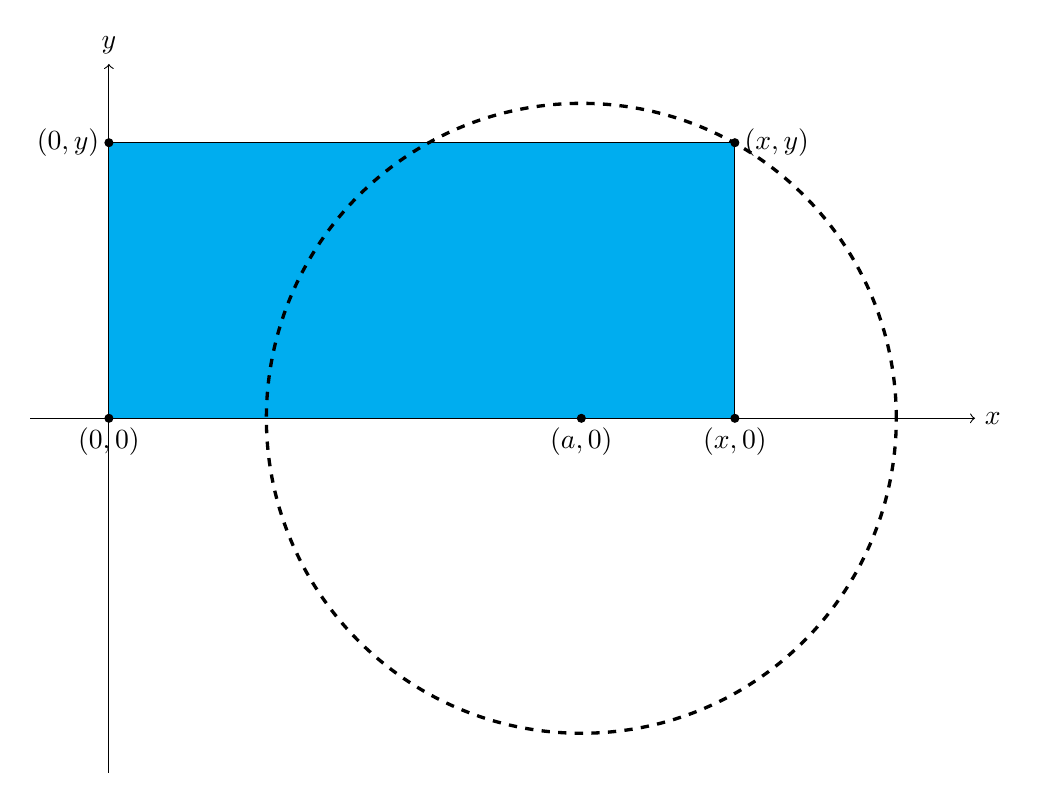
\begin{tikzpicture}
	%\draw[help lines, color=gray!30, dashed] (-2.9,-2.9) grid (4.9,4.9);
	\draw[->] (-1,0)--(11,0) node[right]{$x$};
	\draw[->] (0,-4.5)--(0,4.5) node[above]{$y$};

	
	\filldraw[draw=black,fill=cyan] (0,0) rectangle (7.95,3.5);
	\draw[fill] (7.95,3.5) circle [radius=0.05cm];
	\draw[fill] (0,3.5) circle [radius=0.05cm];
	\draw[fill] (0,0) circle [radius=0.05cm];
	\draw[fill] (7.95,0) circle [radius=0.05cm];
	\draw[fill] (6,0) circle [radius=0.05cm];
	\node[right] at (7.95,3.5) {$ (x, y) $};
	\node[left] at (0,3.5) {$ (0, y) $};
	\node[below] at (0,0) {$ (0, 0) $};
	\node[below] at (7.95,0) {$ (x, 0) $};
	\node[below] at (6,0) {$ (a, 0) $};
	\draw[very thick,dashed] (6,0) circle (4cm);
	\end{tikzpicture}
\end{center}
Die Fläche eines Rechtecks mit den Seiten $ x $ und $ y $ berechnet sich durch
\begin{align*}
f(x,y) = x \cdot y.
\end{align*}
Damit ist unser Ziel die Extremstellen der Funktion $ f $ unter der Nebenbedingung $ \varphi(x,y) = 0 $ zu finden.\\
\\
\underline{2. Finde mögliche Kandidaten für Extrempunkte}\\
Da wir ein Extremwertproblem unter einer Nebenbedingung vorliegen haben, wenden wir das Lagrange Verfahren an. Die Lagrangefunktion ist gegeben durch
\begin{align*}
F(x,y,\lambda) = 
f(x,y) + \lambda \varphi(x,y) = xy + \lambda ( (x-a)^2 + y^2 -16 ). 
\end{align*}
Die notwendigen Bedingung für eine Extremstelle von $ f  $ unter der Nebenbedingung $ \varphi(x,y) = 0 $ ist, dass alle partiellen Ableitungen gleich Null sind. Damit gilt:
\begin{align*}
F_x(x,y,\lambda) = 0 \quad &\Rightarrow \quad y + 2 \lambda (x-a) = 0 \qquad \qquad  \ \  \textrm{(I)} \\
F_y(x,y,\lambda) = 0 \quad &\Rightarrow \quad x + 2 \lambda y = 0 \qquad \qquad \qquad \ \ \  \textrm{(II)}\\
F_\lambda(x,y,\lambda) = 0 \quad &\Rightarrow \quad (x-a)^2 +y^2 -16 = 0 \qquad \textrm{(III)}.
\end{align*}
Diese Bedingungen nennen wir auch Lagrangebedingungen.
Aus der ersten Gleichung erhalten wir
\begin{align*}
y + 2 \lambda (x-a) = 0  
\ \Leftrightarrow \
2 \lambda (x-a) = -y
\ \Leftrightarrow \
2 \lambda =  -\frac{y}{x-a}
\end{align*}
und die Gleichung (II) liefert 
\begin{align*}
x + 2 \lambda y = 0 
\ \Leftrightarrow \
2\lambda y = - x 
\ \Leftrightarrow \ 
2 \lambda = -\frac{x}{y}.
\end{align*}
Wegen $ 2 \lambda = 2 \lambda $ erhalten wir
%Damit erhalten wir
\begin{align*}
 -\frac{y}{x-a} =  -\frac{x}{y}
\ \Leftrightarrow \
\underbrace{y^2 = x (x-a)}_{\textrm{(IV)}}. 
\end{align*}
Wenn wir dies in die Gleichung (III) einsetzen folgt 
\begin{align*}
(x-a)^2 +y^2 -16= (x-a)^2 + x(x-a) - 16 
&=
x^2 -2ax + a^2 + x^2 - ax - 16\\
&=
2x^2 - 3ax + a^2 - 16
= 0.
\end{align*}
Dies ist eine quadratische Gleichung. Durch die Mitternachts-Formel erhalten wir die Lösungen
\begin{align*}
x_{\nicefrac{1}{2}} 
&=
\frac{3a \pm \sqrt{(3a)^2 -4 \cdot 2 (a^2 - 16)}}{2 \cdot 2}
=
\frac{3a \pm \sqrt{9a^2 -8 a^2 + 8 \cdot 16}}{4}
=
\frac{3a \pm \sqrt{a^2 + 128}}{4}\\
\qquad
\Rightarrow 
x_1 
&=
\frac{3a + \sqrt{a^2 + 128}}{4}, \qquad
x_2
=
\frac{3a - \sqrt{a^2 + 128}}{4}.
\end{align*}
Wegen 
\begin{align*}
x_2
=
\frac{3a - \sqrt{a^2 + 128}}{4} < \frac{3a - \sqrt{a^2 }}{4}  = \frac{3a -a }{4} = \frac{2a}{4} = \frac{a}{2}
\end{align*}
gilt $ x_2 \in ( 0, \frac{a}{2}) $. Damit verletzt $ x_2 $ die Gleichung (IV), denn
\begin{align*}
y^2 = x (x - a) < 0 
\end{align*}
ist ein Widerspruch $ (y^2 > 0) $.
Also bleibt $ x_1  $ als einzige Möglichkeit übrig.
Mit der Gleichung (IV) und $ x := x_1 $ gilt dann
\begin{align*}
y^2 = x (x-a)
&= 
\frac{3a + \sqrt{a^2 + 128}}{4}
 \left(\frac{3a + \sqrt{a^2 + 128}}{4} - a \right)
=
\frac{3a + \sqrt{a^2 + 128}}{4}
 \cdot \frac{3a + \sqrt{a^2 + 128}  -4a}{4}\\
&=
\frac{3a + \sqrt{a^2 + 128}}{4}
\cdot \frac{-a + \sqrt{a^2 + 128} }{4}  
=
\frac{-3a^2 + 3a \sqrt{a^2 + 128} - a \sqrt{a^2 + 128} + a^2 +128  }{16}\\
&=
\frac{128  + 2a \sqrt{a^2 + 128} -2 a^2  }{16}\\
&=
\frac{64  + a \sqrt{a^2 + 128} - a^2  }{8}\\
\ \overset{y > 0}{\Rightarrow} \ 
y &= \sqrt{\frac{64  + a \sqrt{a^2 + 128} - a^2  }{8}}.
\end{align*}
Damit ist der Punkt
\begin{align*}
\left(\frac{3a + \sqrt{a^2 + 128}}{4}, \sqrt{\frac{64  + a \sqrt{a^2 + 128} - a^2  }{8}}. \right)
\end{align*}
der einzige Kandidat für ein Extrempunkt von $ f $ unter der Nebenbedingung $ \varphi(x,y) = 0 $.
%Wir konzentrieren uns nun wieder auf den Abstand zwischen $ (a,0) $ und $ (x,y) $.
%Hierfür gilt wegen $ y > 0 $
%\begin{align*}
%y^2 = 4^2 - (x-a)^2 \ \Leftrightarrow \
%y = y(x) = \sqrt{16 - (x-a)^2} . 
%\end{align*}
%Damit lässt sich die $ y$ - Koordinate auf dem oberen Halbkreis durch $ x $ mit $ -4 \leq  x-a  \leq 4 $ darstellen. 
%Insbesondere können wir den Flächeninhalt von $ R $ dann durch
%\begin{align*}
%f(x) = x \cdot y(x) = 
%x \cdot \sqrt{16 - (x-a)^2}
%\end{align*}
%berechnen.
%Die Ableitung von $ f $ ist für $ -4 <  x-a  < 4 $ durch
%\begin{align*}
%f^\prime(x)
%&= y(x) + x \cdot \frac{1}{2 \sqrt{16 - (x-a)^2}} \cdot (-2) (x-a)
%=
%\sqrt{16 - (x-a)^2} - \frac{ x^2 - ax}{\sqrt{16 -(x-a)^2}}\\
%&=
%\frac{16 - (x-a)^2}{\sqrt{16 - (x-a)^2}}  - \frac{ x^2 - ax}{\sqrt{16 -(x-a)^2}}\\
%&=
%\frac{16 -x^2 + 2ax -a^2 - x^2 + ax}{\sqrt{16 - (x-a)^2}}\\
%&=
%\frac{-2x^2  + 3 ax + 16 -a^2}{\sqrt{16 - (x-a)^2}}
%\end{align*}

\newpage